\documentclass[10pt,a4paper]{article}

\renewcommand{\familydefault}{\sfdefault} % new font
% !TeX spellcheck = en_UK

\usepackage[margin=2cm]{geometry}
\usepackage{marvosym}  % symbols
\usepackage{graphicx}
% Defining of two columns with grey line in between
\usepackage{array, xcolor}
\definecolor{lightgray}{gray}{0.8} %Definition of the colour
\newcolumntype{L}{>{\raggedleft}p{0.06\textwidth}} % Definition of the width of left column
\newcolumntype{R}{p{0.9\textwidth}} % right column
\newcommand\VRule{\color{lightgray}\vrule width 0.5pt} % Definition of the new command
% creation of hyperlink
\usepackage[hidelinks]{hyperref}
% redefining of section title
\usepackage{titlesec}
\titleformat{\section}{\Large}{}{0em}{}[\titlerule]
\setlength\parindent{0pt}
\usepackage{skak}  % icons of a bicycle, ball, etc...
\usepackage{tabulary}

%\usepackage{fontspec}
\usepackage{fontawesome}

\usepackage{progressbar}

\usepackage[version=4]{mhchem}

\begin{document}

% take out page number
%\thispagestyle{empty}

\begin{center}
{\Large \textit{CURRICULUM VITAE}}
\end{center}


\begin{minipage}{0.69\textwidth}

\textbf{\huge Fyodor M. Dostoevsky}\\

\vspace{0.1cm}

\large\upshape
\begin{tabular}{ll}
\MVAt & \href{mailto:yourmail@domain.com}{\textcolor[rgb]{0.02,0.02,0.33}{yourmail@domain.com}} \\
\Telefon & (+49) 123456789 \\
\Letter & Moscow, Russian Empire\\
\faMapMarker & 11.11.1821\\
\faLinkedin & \href{https://www.linkedin.com/in/yourlinkedin/}{\textcolor[rgb]{0.02,0.02,0.33}{www.linkedin.com/in/yourlinkedin/}} \\

%\faGithub & github pages here  \vspace{0.2cm}\\

\end{tabular}

\end{minipage}%
\begin{minipage}{0.3\textwidth}
\begin{flushright}
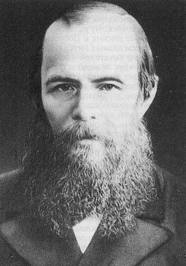
\includegraphics[width=0.5\textwidth]{fyodor_dostoevsky.jpg}
\end{flushright}
\end{minipage}

\section*{\textbf{WORK EXPERIENCE}}
\begin{tabular}{L!{\VRule}R}
1871&
\textbf{Independent writer}\\
1875&\href{https://www.google.com/}{\textcolor[rgb]{0.02,0.02,0.33}{Dostoevsky Publishing Company}}, Saint Petersburg, Russia\vspace{2pt}\\
& "Demons" project \\
& "A Writer's Diary" project\vspace{5pt}\\

01.1843&
\textbf{Field engineer second lieutenant}\\
06.1844&\href{https://www.google.com/}{\textcolor[rgb]{0.02,0.02,0.33}{Firm Name}}, Saint Petersburg, Russia\vspace{2pt}\\
& Boring project
Second boring project\vspace{5pt}\\


\end{tabular}


\section*{\textbf{MANAGEMENT}}

Gambling Experience (Wiesbaden, 1863)\\
Siberian Prison Camp (1849-1854)

\section*{\textbf{SIDE-PROJECTS \& ENGAGEMENTS}}
\begin{tabular}{L!{\VRule}R}
01.2000 & Side Project 1\\
01.2000 & Side Project 2\\

\end{tabular}


\section*{\textbf{EDUCATION}}
\begin{tabular}{L!{\VRule}R}


09.1837&
\textbf{M. Sc.} Military Engineer, Some Faculty, \\
05.1840& \href{https://en.wikipedia.org/wiki/Military_Engineering-Technical_University}{\textcolor[rgb]{0.02,0.02,0.33}{Nikolayev Military Engineering Institute}}, City, Country\vspace{2pt}\\
 &\textit{Thesis}: No Thesis Name\\
 &\textit{Supervisor}: Prof. Noname\vspace{2pt}\\
 & Description 1\\
 & Description 2\\
 & Description 3
 \vspace{5pt}\\

\end{tabular}

\section*{\textbf{SKILLS}}

\begin{tabular}{p{3cm}|p{12cm}}
Writing & god level \\
Psychology & sudo level \\
Philosophy & sudo level \\
Influencer & advanced \\

\end{tabular} 

\section*{\textbf{LANGUAGES}}

German (fluent), English (fluent), French (native) \\

\section*{\textbf{AWARDS \& SCHOLARSHIPS}}
\begin{tabular}{L!{\VRule}R}

1849&
Katorga Award
\vspace{2pt}\\

1956&
olive-green postage stamp of Soviet Union \vspace{2pt}\\

1971&
Own Museum Award \vspace{2pt}\\

\end{tabular}

\section*{\textbf{PUBLICATIONS}}

\textbf{Author}, Author2, A. (2000) Journal Name, Vol. 100, 88-104.\\

\section*{\textbf{WORKSHOPS \& CONFERENCES}}

\subsection*{Presentations}
\begin{tabular}{L!{\VRule}R}
01.2000 & Some Workshop on Stuff (City, Country)\\
... & ...\\
\end{tabular}

\end{document}
